\newpage
\section{Question 3}
	\subsection*{DH Notation}
	\noindent
		\begin{table}[position = here]
		\begin{centering}
		\begin{tabular}{||l|l|l|l|l||}
			\hline \rule[-2ex]{0pt}{5.5ex} \color{red}\bf{i} & \color{red}\bf{$\theta$}		&	\color{red}\bf{d}	&	\color{red}\bf{r}	&	\color{red}\bf{$\alpha$}\\ 
			\hline \rule[-2ex]{0pt}{5.5ex} 1 & $\theta_{1}$	&	67	&	100	&	$\pi/2$	\\	
			\hline \rule[-2ex]{0pt}{5.5ex} 2 & $\theta_{2}$	&	0	&	250	&	0		\\
			\hline \rule[-2ex]{0pt}{5.5ex} 3 & $\theta_{2}$	&	0	&	0	&	$\pi/2$	\\
			\hline \rule[-2ex]{0pt}{5.5ex} 4 & $\theta_{4}$	&	0	&	250	&	$-\pi/2$ \\
			\hline \rule[-2ex]{0pt}{5.5ex} 5 & $\theta_{5}$	&	0	&	0	&	$-\pi/2$	\\
			\hline \rule[-2ex]{0pt}{5.5ex} 6 & $\theta_{6}$	&	0	&	245	&	0		\\
			\hline 
		\end{tabular}\\
		\end{centering}
		\begin{flushleft}
		\caption [DHVariables] {D-H Variable Notation}
		\end{flushleft}
		\end{table}
		
		
		\begin{figure}[position = here]
			\begin{centering}
				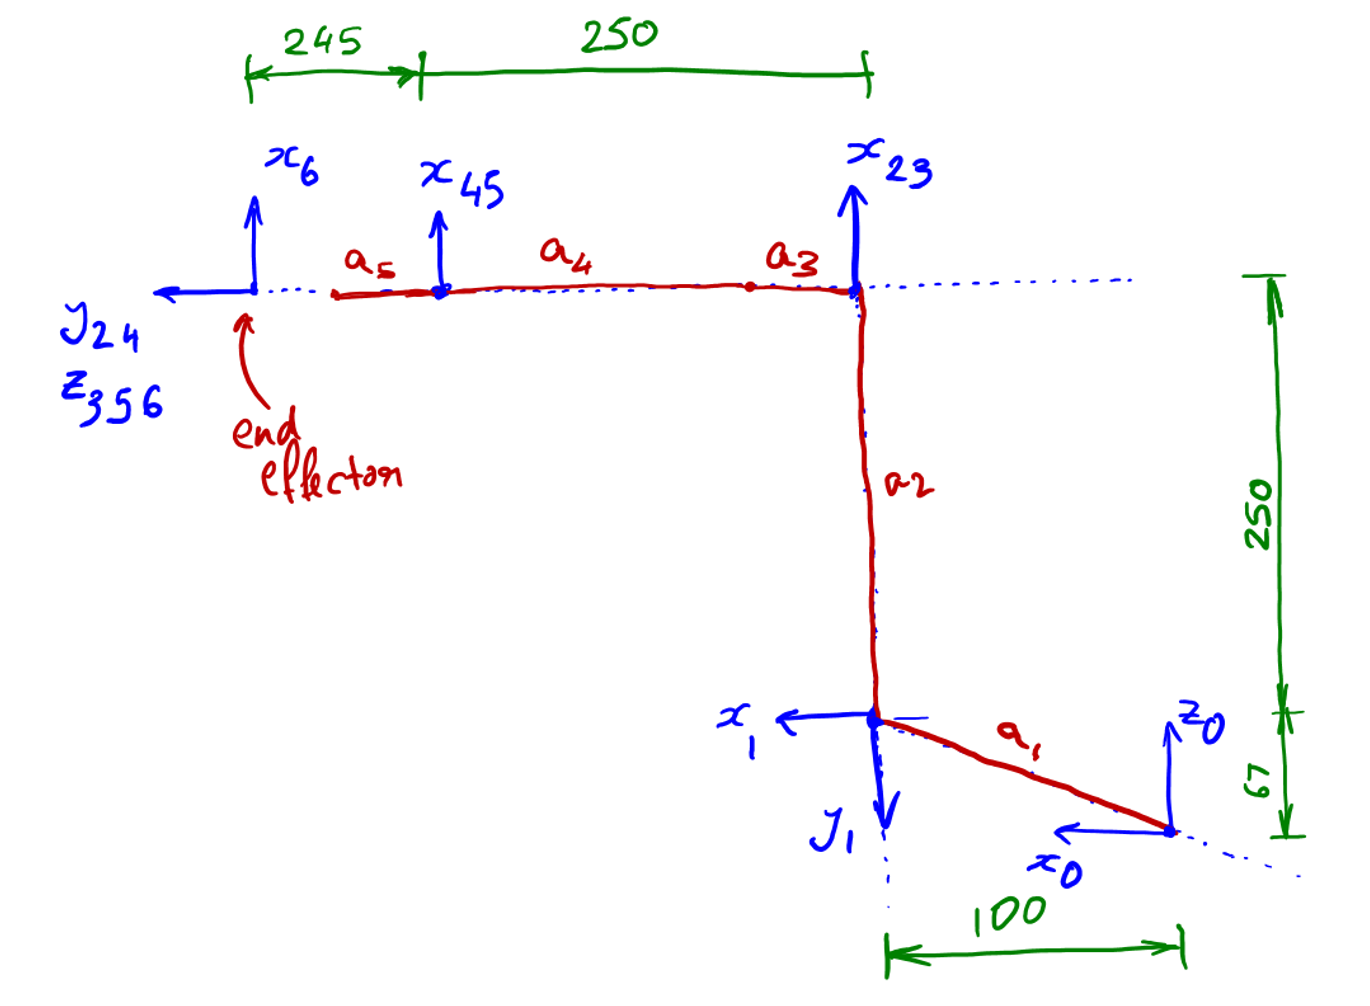
\includegraphics[scale=0.5]{q3}\\
				\caption [DHDrawing]{D-H Standard for Forward Kinematics Coordinate Systems}
			\end{centering}
		\end{figure}
		
	\pagebreak
	\subsection*{Assumption}
	Effectively taking the zero coordinate system above joint J1 allows us to eliminate one transformation from the system without drastically altering the kinematic solution behind it. The solution I provide below will be the transformation matrix with respect to my coordinate system 0.
	
	\subsection*{Code Listing}
	See Appendix A [9.3]
	
	\subsection*{Resulting Transformation Matrix}
	The resulting transformation matrix can be represented as:\\
		\begin{center}
			$$
			\bf{^{0}T_{6}} =
			\begin{pmatrix}
				n_{x} & s_{x} & a_{x} & p_{x}\\
				n_{y} & s_{y} & a_{y} & p_{y}\\
				n_{z} & s_{z} & a_{z} & p_{z}\\
				0	&	0	&	0	&	1
			\end{pmatrix}
			= {^{0}A_{1}} {^{1}A_{2}} {^{2}A_{3}} {^{3}A_{4}} {^{4}A_{5}} {^{5}A_{6}}
			$$
		\end{center}
		\vspace{5mm}
	\flushleft
\bf{n_{x}} =
$$
- \sin\theta_{6} (\cos\theta_{4} \sin\theta_{1} - \sin\theta_{4} (\cos\theta_{1} \sin\theta_{2} \sin\theta_{3} - \cos\theta_{1} \cos\theta_{2} \cos\theta_{3}))-  \cos\theta_{6} (\cos\theta_{5} (\sin\theta_{1} \sin\theta_{4} + \cos\theta_{4} (\cos\theta_{1} \sin\theta_{2} \sin\theta_{3} - \cos\theta_{1} \cos\theta_{2} \cos\theta_{3})) + \sin\theta_{5} (\cos\theta_{1} \cos\theta_{2} \sin\theta_{3} + \cos\theta_{1} \cos\theta_{3} \sin\theta_{2}))
$$\vspace{3mm}

\bf{s_{x}} = 
$$
\sin\theta_{6} (\cos\theta_{5} (\sin\theta_{1} \sin\theta_{4} + \cos\theta_{4} (\cos\theta_{1} \sin\theta_{2} \sin\theta_{3} - \cos\theta_{1} \cos\theta_{2} \cos\theta_{3})) + \sin\theta_{5} (\cos\theta_{1} \cos\theta_{2} \sin\theta_{3} + \cos\theta_{1} \cos\theta_{3} \sin\theta_{2})) - \cos\theta_{6} (\cos\theta_{4} \sin\theta_{1} - \sin\theta_{4} (\cos\theta_{1} \sin\theta_{2} \sin\theta_{3} - \cos\theta_{1} \cos\theta_{2} \cos\theta_{3}))
$$\vspace{3mm}


\bf{a_{x}} =
$$
\sin\theta_{5} (\sin\theta_{1} \sin\theta_{4} + \cos\theta_{4} (\cos\theta_{1} \sin\theta_{2} \sin\theta_{3} - \cos\theta_{1} \cos\theta_{2} \cos\theta_{3})) - \cos\theta_{5} (\cos\theta_{1} \cos\theta_{2} \sin\theta_{3} + \cos\theta_{1} \cos\theta_{3} \sin\theta_{2})
$$\vspace{3mm}

\bf{p_{x}} = 
$$
100 \cos\theta_{1} + 250 \cos\theta_{1} \cos\theta_{2} - 250 \sin\theta_{1} \sin\theta_{4} - 250 \sin\theta_{6} (\cos\theta_{4} \sin\theta_{1} - \sin\theta_{4} (\cos\theta_{1} \sin\theta_{2} \sin\theta_{3} - \cos\theta_{1} \cos\theta_{2} \cos\theta_{3})) - 250 \cos\theta_{6} (\cos\theta_{5} (\sin\theta_{1} \sin\theta_{4} + \cos\theta_{4} (\cos\theta_{1} \sin\theta_{2} \sin\theta_{3} - \cos\theta_{1} \cos\theta_{2} \cos\theta_{3})) + \sin\theta_{5} (\cos\theta_{1} \cos\theta_{2} \sin\theta_{3} + \cos\theta_{1} \cos\theta_{3} \sin\theta_{2})) - 250 \cos\theta_{4} (\cos\theta_{1} \sin\theta_{2} \sin\theta_{3} - \cos\theta_{1} \cos\theta_{2} \cos\theta_{3})
$$\vspace{3mm}

\bf{n_{y}} =
$$
\sin\theta_{6} (\cos\theta_{1} \cos\theta_{4} + \sin\theta_{4} (\sin\theta_{1} \sin\theta_{2} \sin\theta_{3} - \cos\theta_{2} \cos\theta_{3} \sin\theta_{1})) + \cos\theta_{6} (\cos\theta_{5} (\cos\theta_{1} \sin\theta_{4} - \cos\theta_{4} (\sin\theta_{1} \sin\theta_{2} \sin\theta_{3} - \cos\theta_{2} \cos\theta_{3} \sin\theta_{1})) - \sin\theta_{5} (\cos\theta_{2} \sin\theta_{1} \sin\theta_{3} + \cos\theta_{3} \sin\theta_{1} \sin\theta_{2}))
$$\vspace{3mm}



\bf{s_{y}} =
$$
\cos\theta_{6} (\cos\theta_{1} \cos\theta_{4} + \sin\theta_{4} (\sin\theta_{1} \sin\theta_{2} \sin\theta_{3} - \cos\theta_{2} \cos\theta_{3} \sin\theta_{1})) - \sin\theta_{6} (\cos\theta_{5} (\cos\theta_{1} \sin\theta_{4} - \cos\theta_{4} (\sin\theta_{1} \sin\theta_{2} \sin\theta_{3} - \cos\theta_{2} \cos\theta_{3} \sin\theta_{1})) - \sin\theta_{5} (\cos\theta_{2} \sin\theta_{1} \sin\theta_{3} + \cos\theta_{3} \sin\theta_{1} \sin\theta_{2}))
$$\vspace{3mm}

\bf{a_{y}} = 
$$
- \sin\theta_{5} (\cos\theta_{1} \sin\theta_{4} - \cos\theta_{4} (\sin\theta_{1} \sin\theta_{2} \sin\theta_{3} - \cos\theta_{2} \cos\theta_{3} \sin\theta_{1})) - \cos\theta_{5} (\cos\theta_{2} \sin\theta_{1} \sin\theta_{3} + \cos\theta_{3} \sin\theta_{1} \sin\theta_{2})
$$\vspace{3mm}

\bf{p_{y}} =
$$
100 \sin\theta_{1} + 250 \cos\theta_{2} \sin\theta_{1} + 250 \cos\theta_{1} \sin\theta_{4} + 250 \sin\theta_{6} (\cos\theta_{1} \cos\theta_{4} + \sin\theta_{4} (\sin\theta_{1} \sin\theta_{2} \sin\theta_{3} - \cos\theta_{2} \cos\theta_{3} \sin\theta_{1})) - 250 \cos\theta_{4} (\sin\theta_{1} \sin\theta_{2} \sin\theta_{3} - \cos\theta_{2} \cos\theta_{3} \sin\theta_{1}) + 250 \cos\theta_{6} (\cos\theta_{5} (\cos\theta_{1} \sin\theta_{4} - \cos\theta_{4} (\sin\theta_{1} \sin\theta_{2} \sin\theta_{3} - \cos\theta_{2} \cos\theta_{3} \sin\theta_{1})) - \sin\theta_{5} (\cos\theta_{2} \sin\theta_{1} \sin\theta_{3} + \cos\theta_{3} \sin\theta_{1} \sin\theta_{2}))
$$\vspace{3mm}

\bf{n_{z}} = 
$$
\cos\theta_{6} (\sin\theta_{5} (\cos\theta_{2} \cos\theta_{3} - \sin\theta_{2} \sin\theta_{3}) + \cos\theta_{4} \cos\theta_{5} (\cos\theta_{2} \sin\theta_{3} + \cos\theta_{3} \sin\theta_{2})) - \sin\theta_{4} \sin\theta_{6} (\cos\theta_{2} \sin\theta_{3} + \cos\theta_{3} \sin\theta_{2})
$$\vspace{3mm}

\bf{s_{z}} = 
$$
- \sin\theta_{6} (\sin\theta_{5} (\cos\theta_{2} \cos\theta_{3} - \sin\theta_{2} \sin\theta_{3}) + \cos\theta_{4} \cos\theta_{5} (\cos\theta_{2} \sin\theta_{3} + \cos\theta_{3} \sin\theta_{2})) - \cos\theta_{6} \sin\theta_{4} (\cos\theta_{2} \sin\theta_{3} + \cos\theta_{3} \sin\theta_{2})
$$\vspace{3mm}

\bf{a_{z}} = 
$$
\cos\theta_{5} (\cos\theta_{2} \cos\theta_{3} - \sin\theta_{2} \sin\theta_{3}) - \cos\theta_{4} \sin\theta_{5} (\cos\theta_{2} \sin\theta_{3} + \cos\theta_{3} \sin\theta_{2})
$$\vspace{3mm}

\bf{p_{z}} = 
$$
250 \sin\theta_{2} + 250 \cos\theta_{6} (\sin\theta_{5} (\cos\theta_{2} \cos\theta_{3} - \sin\theta_{2} \sin\theta_{3}) + \cos\theta_{4} \cos\theta_{5} (\cos\theta_{2} \sin\theta_{3} + \cos\theta_{3} \sin\theta_{2})) + 250 \cos\theta_{4} (\cos\theta_{2} \sin\theta_{3} + \cos\theta_{3} \sin\theta_{2}) - 250 \sin\theta_{4} \sin\theta_{6} (\cos\theta_{2} \sin\theta_{3} + \cos\theta_{3} \sin\theta_{2}) + 67
$$\vspace{3mm}
\end{center}

\pagebreak
\subsection*{World Coordinate Transformation}
 If it is necessary to calculate the transformation matrix with respect to the "real" (0, 0, 0) world coordinate system (as defined by the assignment document) we can take the following matrix:


		$$
		\bf{^{W}A_{0}} =
		\begin{pmatrix}
		0 & -1 & 0 & 0\\
		1 & 0  & 0 & 253\\
		0 & 0  & 1 & 0\\
		0 &	0  & 0 & 1
		\end{pmatrix}
		$$

and multiply it with our Transformation Matrix ${^{0}T_{6}}$:\\
\vspace{10mm}
$	{^{W}T_{6}} = {^{W}A_{0}}\cdot {^{0}T_{6}}	=$	
								\begin{left}
									$$
									\begin{pmatrix}
									0 & -1 & 0 & 0\\
									1 & 0  & 0 & 253\\
									0 & 0  & 1 & 0\\
									0 &	0  & 0 & 1
									\end{pmatrix} \cdot
								\end{left}
								\begin{right}
									\begin{pmatrix}
									n_{x} & s_{x} & a_{x} & p_{x}\\
									n_{y} & s_{y} & a_{y} & p_{y}\\
									n_{z} & s_{z} & a_{z} & p_{z}\\
									0	&	0	&	0	&	1
									\end{pmatrix}
									$$
								\end{right}\\
\vspace{10mm}
${^{W}T_{6}}$ = 
					\begin{right}
						$$
						\begin{pmatrix}
							-n_{y} & -s_{y} & a_{y} & p_{y}\\
							n_{x} & s_{x} & a_{x} & p_{x}+253\\
							n_{z} & s_{z} & a_{z} & p_{z}\\
							0	&	0	&	0	&	1
						\end{pmatrix}
						$$
					\end{right}\\
					\vspace{5mm}
This can be used for inverse kinematics problems by substituting our end effector position values into ${^{W}T_{6}}$ in order to calculate the joint angles. We will see more about this in Question 6.